\documentclass[notitlepage]{article}
\usepackage{color,soul,amsmath,graphicx}
\usepackage[outercaption]{sidecap}
\usepackage[citestyle=numeric,backend=bibtex]{biblatex}
\usepackage[font=small,labelfont=bf]{caption}
\usepackage{verbatim}
\sidecaptionvpos{figure}{c}
\providecommand{\abs}[1]{\lvert#1\rvert}
\providecommand{\norm}[1]{\lVert#1\rVert}
\bibliography{library}
\immediate\write18{python proteome-analysis.py}

\title{Increased concentration of proteins with growth rate can result from passive resource redistribution}
\begin{comment}
\author{Leeat Keren, Uri Barenholz, Ron Milo}
\end{comment}

\begin{document}
\maketitle
\abstract{
  In many microorganisms, the proteome composition changes dramatically as a function of the growth environment.
Furthermore, many of these changes seem to be coordinated with the growth rate rather than the specific environment.
However, although cellular growth rates, gene expression levels and gene regulation have been at the center of biological research for decades, their quantitative interdependence is not yet fully understood.

We analyzed the relationship between growth rate and proteome composition for the model microorganism \emph{E.coli} as reflected in two recently published proteomics data sets spanning various growth conditions.
We found that the cellular concentration of a large fraction of the proteins measured coordinately increases with the growth rate.
This fraction includes proteins spanning different functional groups and proteins that are involved in different cellular processes.
Notably, ribosomal proteins are only a small fraction of this group of proteins.
We present a simple model that demonstrates how such a widely coordinated increase in the concentration of many proteins can be the result of passive redistribution of resources, due to active regulation of only a few proteins.
Our model provides a potential explanation for why and how there is a global coordinated response of a large fraction of the proteome to the growth rate under different environmental conditions.
Its simplicity can also be useful by serving as a baseline null hypothesis in the search for active regulation.

We suggest that, although the concentrations of many proteins change with the growth rate, such changes could be part of a global effect, not requiring specific cellular control mechanisms.
}

\section{Introduction}
A fundamental system-level challenge for cell physiology is the achievement of proper function in the face of various environmental conditions.
It has been established for many years that in different environments cells differ in many properties, including their shape, size, growth rate, and macro-molecular composition \parencite{Schaechter1958, Maaloe1969, Churchward1982, Pedersen1978a, ingraham1983growth,Bremer1987}, with strong interdependence between these parameters.

Early on it was found that the expression of some genes is coordinated with growth rate, rather than with the specific environment.
Classical experiments in bacteria, by researchers from what became known as the Copenhagen school, have shown that ribosome concentration (inferred from the RNA to protein ratio in cells) increases in proportion to growth rate\parencite{Schaechter1958}.
The search for mechanisms in \emph{E.coli} that underlie this observation yielded several candidates.
Specifically, coordination between ribosome production and growth rate was attributed both to the pools of purine nucleotides \parencite{Gourse1996,Gaal1997}, and the tRNA pools through the stringent response \parencite{Chatterji2001,Brauer2008a}.
For a more thorough review see \parencite{Nomura1984}.
The logic behind this observed increase is that, given that translation rates and ribosome functional fraction remain relatively constant across conditions, a larger fraction of ribosomes out of the proteome is needed in order to achieve faster growth \parencite{neidhardt1999a,dennis2004,Zaslaver2009}.

In the last two decades, with the development of the ability to measure genome-wide expression levels, it was found that coordination of gene expression (measured through mRNA levels and promoter-reporter libraries) and growth rate is not limited to ribosomes and ribosomal genes.
In \emph{E.coli}, the expression of catabolic and anabolic genes is coordinated with growth rate, and suggested to be mediated by cAMP \parencite{Saldanha2004}.
In \emph{S.cerevisiae}, it was shown that a surprisingly large fraction of the genome changes its expression levels in response to environmental conditions in a manner strongly correlated with growth rate \parencite{Keren2013a,Gasch2000,Castrillo2007,Zaslaver2009, Gerosa2013}.
Studies examining the interplay between global and specific modes of regulation, suggested that global factors play a major role in determining the expression levels of genes \parencite{Gasch2000, Klumpp2009a,Scott2010, Berthoumieux2013}.
In \emph{E.coli}, this was mechanistically attributed to changes in the pool of RNA polymerase core and sigma factors \parencite{Klumpp2008}.
In \emph{S.cerevisiae}, it was suggested that differences in histone modifications around the replication origins \parencite{regenberg2006} or translation rates \parencite{Gasch2000} across conditions may underlie the same phenomenon.
Important advancements in \emph{E.coli} were achieved by analyzing measurements of fluorescent reporters through a simplified model of gene expression built upon the empirical scaling with growth rate of different cell parameters (such as gene dosage, transcription rate and cell size)\parencite{Klumpp2009a}.
These studies suggest that the expression of all genes changes with growth rate, with different architectures of regulatory networks yielding differences in the direction and magnitude of these changes. 

Despite these advancements, many gaps remain in our understanding of the connection between gene expression and growth rate.
Primarily, it is unclear what is the degree of interconnection between gene expression and growth rate.
Is it unique to specific groups of genes or is it a more global phenomenon shared across most genes in the genome?
Genome-wide proteomic data sets, such as those generated by fluorescent fusion proteins or mass-spectrometry, which probe the proteome composition at different growth rates, offer potential insights into these questions.

In this work we analyzed two recently published proteomic data sets of \emph{E.coli} under different growth conditions \parencite{Valgepea2013} [ref unpublished Heinemann].
We find a positive correlation between growth rate and the protein concentration of many genes, from diverse functional groups.
Based on this recently published data we present a baseline model, which does not require fine-tuning according to organism-specific parameters, that quantitatively predicts the relationship between gene regulation, protein abundance and growth rate.
Our model provides a baseline for the behavior of endogenous genes in conditions in which they are not differentially regulated, on top of which different regulatory aspects can be added.
It suggests that positive correlation of protein concentration with growth rate is a system-emerging property that is the result of passive redistribution of resources, without need for specific regulation mechanisms.

\section{Results}
\subsection{Analysis of proteomic data sets}
To examine the interdependence of protein concentration and growth rate across expressed genes we analyzed two published proteomics data sets of \emph{E.coli}, \parencite{Valgepea2013} and [ref Heinemann].
These data sets use mass spectrometry to evaluate the proteomic composition of \emph{E.coli} under $5$ different growth rates using a chemostat, in \parencite{Valgepea2013}, and $13$ different growth conditions, spanning both different carbon sources and chemostat-controlled growth rates, in [ref Heinemann]\footnote{The [ref Heinemann] data set contains more conditions than those analyzed, see section \ref{heinemanncond} for further details}.
\subsubsection{A large fraction of the proteome is positively correlated with growth rate}
For each data set, we measured the Pearson correlation of every protein with the growth rate (Figure \ref{fig:growthcorr}, see Methods section for more details).
We find that a large number of proteins ($724$ out of $1981$ measured in the data set from [ref Heinemann], hereafter referred to as H, and $296$ out of $2184$ in the data set from \parencite{Valgepea2013}, hereafter referred to as V) are significantly positively correlated with the growth rate \footnote{Significant correlation was defined as a correlation above 0.8 for the V data set and a correlation in the range (0.4,0.8) for the H data set, See SI for further discussion}.
Notably, in both data sets, the proteins that have a high correlation with the growth rate are involved in different cellular functions and span different functional groups (To-Do refer to table with breakdown by function).
Specifically, these groups include more proteins than the 56 ribosomal proteins, and the proteins they include are not generally expected to be co-regulated.
For further comparison and analysis of the causes underlying the differences between the two data sets as reflected in Figure \ref{fig:growthcorr} see section \ref{heinemannchemo}

\begin{figure}[h]
\centering
\includegraphics{GrowthRateCorrelation.pdf}
\caption{
A significant fraction of the proteins have positive correlation with the growth rate in the two data sets analyzed (ranges used for high correlation are marked in dashed lines).
These proteins span many functional groups.
The thresholds used for defining high correlation are marked in dashed lines.
(Proteins with unknown function (present in the Heinemann data set, right panel) show less correlation with growth rate, as well as proteins with low levels of expression (data not shown).)
}
\label{fig:growthcorr}
\end{figure}
From this point on, we focus our analysis on this group of significantly positively correlated with growth rate proteins (as defined above).
\subsubsection{Positively correlated with growth rate proteins share a similar response}
\label{propchange}
Following the identification of this group, we wished to examine how similar is the behavior with growth rate for these different proteins.
We note that the fact that two proteins have the same correlation with the growth rate does not imply that they are correlated between themselves.
Moreover, it also does not imply that they scale in the same way with the growth rate.
We therefore calculated the slope of a linear regression line with the growth rate for every one of these protein and plotted the results in Figure \ref{fig:globalfit} (Further details on the calculation are in section \ref{concacrossconds}).
We find that the distribution of estimated slopes falls within the expected range resulting from measurement errors of the proteins concentrations (ToDo: This is not calculated yet!).
This analysis thus reveals that, not only does a significant fraction of the proteome is highly positively correlated with the growth rate, but that, moreover, these proteins respond in a similar manner across the different conditions.

Furthermore, we examined how the response of the highly correlated proteins relates to the well-studied response of ribosomal proteins.
To that end, we performed the same analysis of slopes, restricting it to ribosomal proteins alone (Figure \ref{fig:globalfit}, green bars).
The analysis shows that, on average, highly correlated proteins scale in the same way as ribosomal proteins do, suggesting that the observed response of ribosomes concentration with growth rate is a much more widespread phenomena encompassing many more cellular components.
Moreover, this finding challenges the control mechanisms previously suggested for ribosomal proteins as it demonstrates that either these control mechanisms affect many more proteins, or that another, more general mechanism exists.

\begin{figure}[h]
\centering
\includegraphics{AllProtsVSRibosomalNormalizedSlopes.pdf}
\caption{
    A histogram of the normalized slopes of the trend lines for every high correlation protein (blue), and for every ribosomal protein (green) is shown for the two data sets analyzed.
    Left panel - data from \parencite{Valgepea2013}, right panel - data from \parencite{Heinemann2014}.
    High correlation proteins all share a relatively similar response, meaning they maintain their relative ratios.
    Ribosomal proteins respond in a similar manner to the rest of the high correlation proteins .
    (To-Do confidence intervals or some other heuristic for justifying the observed variation)
}
\label{fig:globalfit}
\end{figure}

\subsubsection{Changes in the proteome across environmental conditions are dominated by proteins that are positively correlated with growth rate}
Lastly, in order to assess the significance of the positive correlation with growth rate of proteins, out of the total change in proteome composition across conditions, we summed the concentrations of all of the proteins that are highly correlated with growth rate across the conditions measured and plotted their total concentration against the growth rate (Figure \ref{fig:globalgrcorr})
(ToDo: consider clustering using PCA or some other method instead of arbitrarily selecting high correlation boundaries, if not then at least add figures demonstrating validity of results even under different boundaries).
Both data sets show that these proteins concentrations change significantly across the different conditions ($\approx 2$ fold change in total concentration across $\approx 5$ fold change of the growth rate).
Moreover, most of the variability of the total concentration of these proteins can be explained by the growth rate ($R^2$ of $0.75$ in H and $0.99$ in V). 
Importantly, the highly correlated proteins form a large fraction of the proteome mass-wise, approaching or exceeding $50\%$ of the proteome at the higher growth rates measured.
Thus, when considering the changes in proteome composition across conditions, we find that, at higher growth rates, $\approx 50\%$ of the proteome composition is determined by the correlation with growth rate of the same group of proteins.
(ToDo: This analysis, unlike the one done in Leeat's work, does not try to identify the scaling between every two conditions and then cluster genes according to conditions where specific regulation occurred, I'm now thinking of ways of modifying this analysis in that direction as it can potentially be much more interesting and strong so generally I believe this paragraph and accompanying figure will be replaced)
For further analysis of the differences between the two data sets see section \ref{heinemannchemo}.

We therefore observe that a large fraction of the change in the proteome composition across conditions is the result of scaling with growth rate of many proteins.
This scaling with growth rate is proportional, maintaining the proteins relative abundances, and encompasses many proteins from different functional groups and cellular mechanisms.

\begin{figure}[h]
\centering
\includegraphics{GlobalClusterGRFit.pdf}
\caption{
The sum of the concentrations of the highly correlated proteins (defined as having a correlation above 0.8 for the V data set and a correlation in the range (0.4,0.8) for the H data set) in each of the data sets, with linear regression lines, is shown.
These proteins form a large fraction out of the proteome at higher growth rates ($>40\%$ for H and $>50\%$ for V).
The change in the concentration of the highly correlated proteins is about 2-fold while the growth rate changes by about 5-fold.
(ToDo: Calculate the estimated degradation rates and/or rate changes as noted in the model, as well as confidence intervals.)
}
\label{fig:globalgrcorr}
\end{figure}


\subsection{Theoretical model}
In an attempt to explain how such a wide-span positive response occurs parsimoniously, we have constructed a minimalistic model that is able to reproduce these results as the outcome of redistribution of resources of the bio-synthesis machinery.
Briefly, the model assumes that favorable growth conditions allow the cell to down-regulate some proteins that are needed in harsher conditions, thus reducing the amount of proteins that need to be produced for the cell to proliferate (Figure \ref{fig:model}).
As a consequence, the fraction of each of the rest of the proteins out of the proteome increases, assuming they are being expressed in the same relative ratios, without invoking specific regulation.
The growth rate therefore increases as well, as the ratio of bio-synthetic machinery to the rest of the proteome increases (Figure \ref{fig:model}B).
To demonstrate the idea concretely, one could think about the down regulation of the lac operon in the presence of Glucose, that alleviates the need to transcribe and translate lactose metabolizing genes and coincides with faster growth.

\begin{figure}[h]
\centering
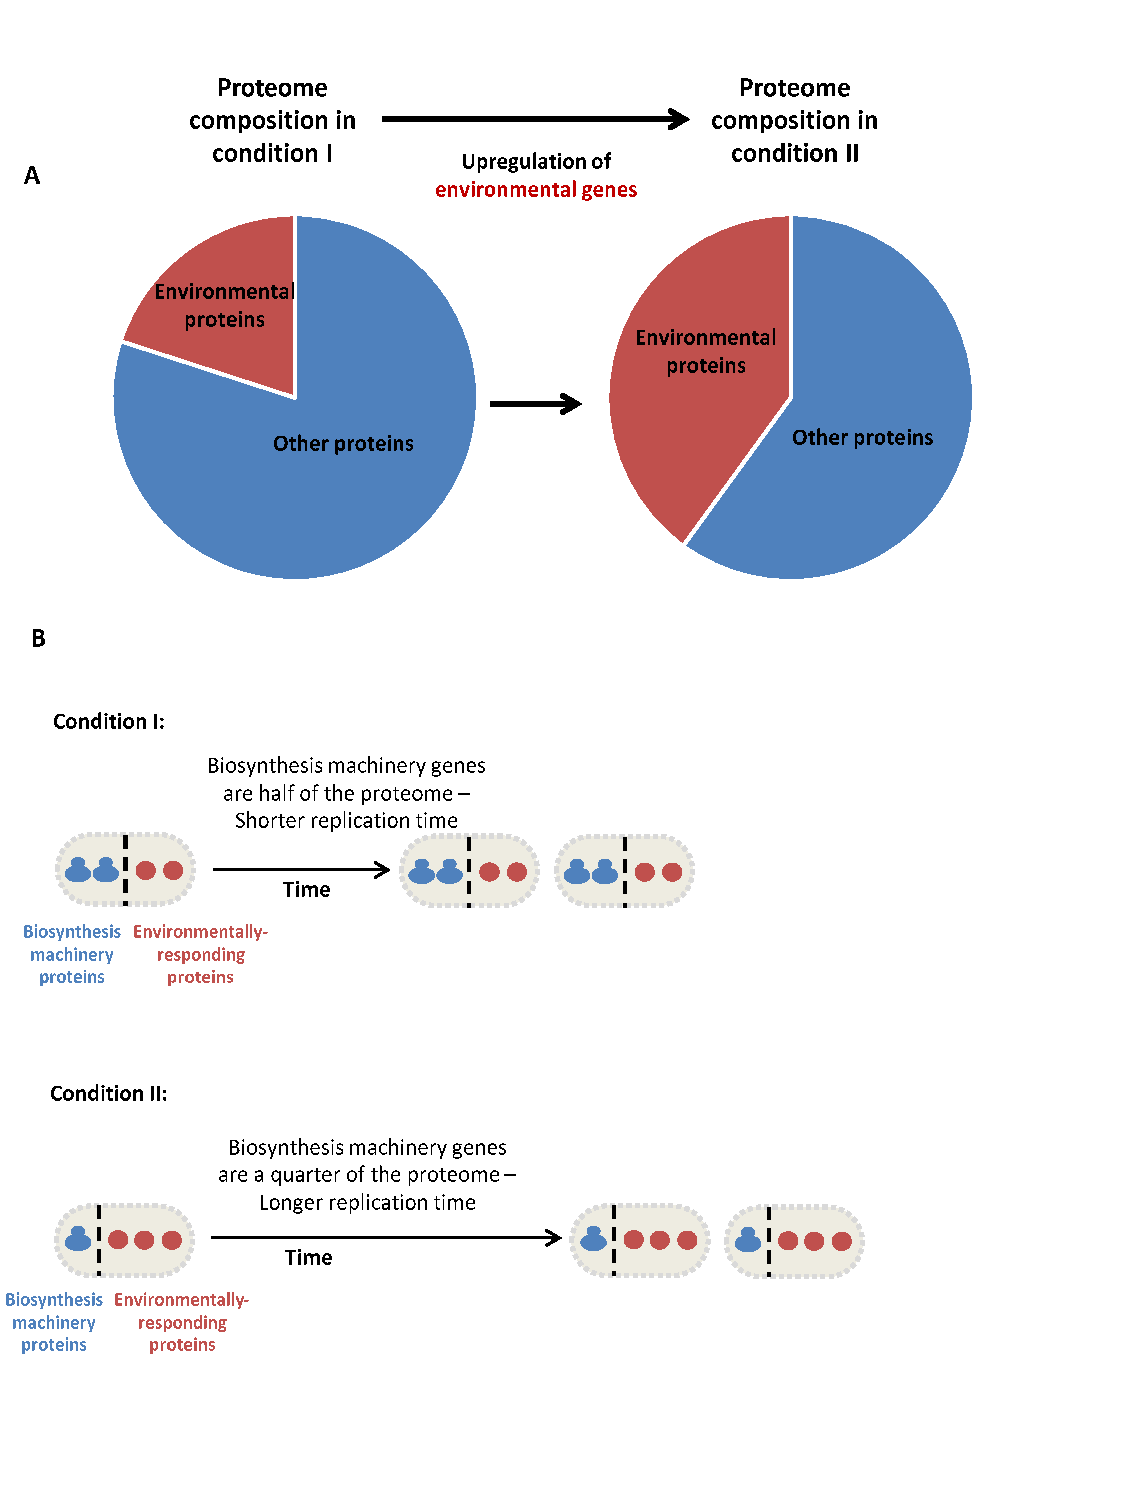
\includegraphics[scale=0.8]{Figures7-trieste.pdf}
\caption{
  A minimalistic model predicts down regulation of environmental genes increases the concentration of other proteins (Panel A).
As a result, the ratio of bio-synthesis machinery genes to the rest of the proteome increases, resulting in faster growth (Panel B).
}
\label{fig:model}
\end{figure}

\subsubsection{The concentration of a protein is determined by both gene specific, and global control of expression}
For every protein, the model decouples its resulting concentration as the product of two control mechanisms:
\begin{enumerate}
\item Protein/gene specific controls such as the associated gene's promoter sequence, 5'-UTRs, ribosomal binding site sequence, and factors affecting this specific gene's expression such as transcription factors and riboswitches that react with the relevant gene.
  While some of these controls (such as, for example, the ribosomal binding sites) are static, and therefore condition independent, others are dynamic and may differ under different environmental conditions (such as transcription factors state).
\item The global state of the cell, including availability of RNA Polymerase, co-factors, Ribosomes, amino-acids etc.
  All of these factors can potentially differ across different environmental conditions.
\end{enumerate}
According to the model, every gene, under every environmental condition, is given an 'affinity-for-expression' (or 'intrinsic-strength') score that encapsulates its gene-specific control state under the condition considered (denoted $w_i(c)$, where $c$ refers to the growth condition).
Our model assumes that the bio-synthetic resources of the cell (Ribosomes, RNA Polymerases, etc.) are distributed among the genes according to their affinities under the condition at hand.
The resulting protein concentration, under a specific condition, is therefore its specific affinity under the condition, divided by the sum of all the affinities of all of the genes under that same condition.
Thus, if two proteins have the same affinity under some condition, they will have the same concentration under that condition, if protein $A$ has twice the affinity of protein $B$ under the same condition, then $A$'s concentration will be twice as high as $B$'s concentration under that condition, etc.

This relationship can be simply formulated as follows:
\begin{equation}
  \label{eq:concentration-ratio}
  p_i(c)=\frac{P_i(c)}{P(c)}=\frac{w_i(c)}{\sum_jw_j(c)}
\end{equation}
where $p_i(c)$ denotes the concentration of protein $i$ under condition $c$, $P_i(c)$ denotes the mass of protein $i$ under condition $c$ per cell, and $P(c)$ denotes the total mass of proteins per cell under condition $c$.

This equation implies that the actual concentration of a protein is determined by two factors, first, obviously, its own specific affinity that is present in the nominator, but second, and less intuitive and commonly thought of, the affinity of all of the other genes under the growth condition, as reflected in the denominator.

\subsubsection{Different growth conditions trigger changes in expression of specific proteins that indirectly affect all of the proteome}
Different environmental conditions may require the expression of different genes in order to achieve growth.
For example, comparing two growth media, one that includes all the required amino-acids (abbreviated as AA), and one that includes none, it can be assumed that when all the AA are present, no need exists for the cell to express AA synthesizing enzymes, whereas when AA's are absent, these enzymes must be expressed.
Therefore, ideally, the cell will be able to sense the presence or absence of AA in the growth media and, for the AA synthesizing genes, down or up regulate their affinities accordingly.
If we now consider some arbitrary protein $i$, whose specific affinity is unaltered between these two conditions, we see that its concentration will most likely still change between the two conditions as the affinities of at least some of the genes (the AA synthesizing enzymes) change, changing the denominator in equation \ref{eq:concentration-ratio} and thus affecting the distribution of resources between all of the expressed genes.

Generalizing this notion, for every group of conditions, one could divide the proteins into those whose intrinsic affinity remains constant across all of the conditions, and to those whose intrinsic affinity changes (meaning their expression is actively regulated by the cell) between at least some of the conditions (see Figure \ref{fig:model}A).
An interesting consequence of the formulation in Equation \ref{eq:concentration-ratio} is that proteins whose intrinsic affinities remain constant across different growth conditions, also maintain their relative concentrations across these conditions with respect to each other.
(ToDo: consider adding a panel to Figure 4 to show this, or sub-slices in the blue slice at 4A, or show by writing the equation for the ratio between to proteins whose affinities remain constant, across different conditions).
Therefore, identifying a large group of proteins that maintain their relative concentrations across conditions (as was identified in section \ref{propchange}) may indicate that these proteins maintained their intrinsic affinities and that any changes in their absolute concentrations are in fact a passive outcome resulting from changes in the intrinsic affinities of other proteins.

\subsubsection{The observed growth rate is an outcome of proteome composition and environmental conditions}
While it is sometimes implied that different cellular components are regulated by the growth rate, here we treat the growth rate as an outcome of the combination of proteome composition and the environmental conditions.
Specifically, we evaluate the growth rate as the result of dividing the total amount of proteins per cell by the amount of bio-synthesis machinery in that cell.
The larger the ratio of total proteins to bio-synthesis proteins is, the longer these bio-synthesis proteins will have to operate in order to duplicate the proteome, and thus the longer the doubling time of the cell will be.

To illustrate this assumption concretely, one could think about the total amount of proteins per cell (measured in AA count) divided by the number of ribosomes in the cell.
Assuming each ribosome translates at an approximately condition-independent rate of about 20 AA per second, and as the amount of actively translating ribosomes is also relatively condition-independent (refs), it follows that the doubling time is linearly dependent on the ratio of proteins to ribosomes in the biomass (see Figure \ref{fig:model}B).

Theoretically, the fastest doubling time a cell may have is the doubling time achieved when all of the cell's proteome is the bio-synthetic machinery.
(ToDo - calculate this time based on known rates and molecular sizes and add to SI)
We denote this minimal doubling time by $T_B$.

To integrate the notion of total protein to bio-synthetic protein ratio into our model, we assume that there is a group of bio-synthetic genes (e.g. genes of the transcriptional and translational machineries) which are not actively differentially regulated across different conditions.
Furthermore, we assume that the machineries these genes are involved at operate at relatively constant rates and occupancy ratios across conditions.
Mathematically we can therefore define this group of bio-synthesis genes, $G_B$, such that, for every gene that belongs to this group, its affinity is constant regardless of the condition:
\begin{equation}
  \label{eq:biosynth-def}
  \forall k \in G_B, c \rightarrow w_k(c)=w_k
\end{equation}

To keep our notations short, we will define the (condition independent) sum over all of these genes as the constant: $W_B = \sum_{k\in G_B}w_k$.

As these genes form the bio-synthesis machinery, and according to the logic presented above, it follows that the doubling time under a given condition, $\tau(c)$ will be linearly proportional to the ratio of total protein to bio-synthesis protein under that condition, with the proportionality constant being $T_B$:
\begin{equation}
  \label{eq:gr-ratio}
  \tau(c) = T_B\frac{P(c)}{\sum_{k\in G_B}P_k(c)}=T_B\frac{\sum_jw_j(c)}{W_B}
\end{equation}
Therefore, the model implies that for conditions that require the expression of larger amounts of non-bio-synthetic genes, the resulting doubling time will be longer, and thus, the growth rate will be lower.

\subsubsection{The concentration of a non-differentially regulated protein is expected to increase with the growth rate} 
Recalling that the connection between the growth rate and the doubling time is: $g(c)=\frac{\ln(2)}{\tau(c)}$, we now combine Equation \ref{eq:concentration-ratio} with Equation \ref{eq:gr-ratio} to get that:
\begin{equation}
  \label{eq:default-response}
  p_i(c)=\frac{w_i(c)}{\sum_jw_j(c)}=\frac{w_i(c)}{W_B}\frac{W_B}{\sum_jw_j(c)}=\frac{w_i(c)}{W_B}\frac{T_B}{\ln(2)}g(c)
\end{equation}

Incorporating all the condition-independent constants ($W_B$, $T_B$, $\ln(2)$) into one term, $C$, we get that the predicted concentration of protein $i$ under condition $c$ is:
\begin{equation}
  \label{eq:final-conc}
  p_i(c)=Cw_i(c)g(c)
\end{equation}
which implies that, for every two conditions between which $i$ maintains its affinity, ($w_i(c_1)=w_i(c_2)$), $i$'s concentration will scale like the growth rate change between these two conditions.

To summarize, the simplistic model we have constructed predicts that, under no specific regulation, the concentration of a protein should scale with the growth rate.
A group of such proteins should therefore maintain their relative concentrations across conditions.
Finally, when the growth rate approaches 0, the concentration of such proteins should also approach 0.

However, as the analysis of experimental data in Figure \ref{fig:globalgrcorr} shows, while the concentration of many proteins does indeed scale linearly with growth rate, this scaling does not imply a drop to 0 concentration at 0 growth.
There are at least two factors that have been neglected in the model, but that can account for this result, and the analysis of their expected effects follows.

\subsubsection{Protein degradation differentiates between measured growth rate and biomass synthesis rate}
Interestingly, accounting for protein degradation affects the expected concentration of non-differentially regulated proteins at 0 growth rate.
Thus, accounting for protein degradation may serve as a partial explanation for the discrepancy between experimental data and the model's predictions.

Assuming that protein degradation acts on all proteins in the same way, and that it is invariant in the growth condition, the effect of protein degradation can be understood as follows: at any time, some fraction of the entire proteome is degraded.
Therefore, the \emph{observed} growth rate, $g$, is, in fact, the amount of proteins produced \emph{minus} the amount of proteins degraded.
To illustrate, if the measured growth rate is 0, the implication is not that no proteins are produced, but rather that proteins are produced at exactly the same rate as they are degraded.

Integrating this notion into the model means that, where the equations previously referred to the observed growth rate, $g$, as the indicator of protein synthesis rate, they should in fact refer to the observed growth rate plus the degradation rate, as that is the real rate of protein synthesis.
Therefore, if we denote by $\alpha$ the degradation rate, Equation \ref{eq:final-conc} should be rewritten as:
\begin{equation}
  \label{eq:final-conc-deg}
  p_i(c)=Cw_i(c)(\alpha+g(c))
\end{equation}
which can now yield better agreement with the experimental results as presented in Figure \ref{fig:globalgrcorr} (depending on the exact value set for degradation), partially explaining why the concentration of non-differentially regulated proteins does not drop to 0 when the growth rate is 0.
(ToDo - add exact predicted degradation rate that achieved good agreement with experimental results)

\subsubsection{Slower biological processes rates at slower growth affect the relation between proteome composition and growth rate}
(ToDo - Note that it is an idea Hwa brought up during our conversation).
The simplistic model assumes that the doubling time is proportional to the ratio of total protein to bio-synthetic protein.
This assumption fails if the rate at which the bio-synthetic machinery operates changes across conditions.
Replacing this assumption by a dependence of bio-synthesis rate with growth rate (such that, the faster the growth, the faster the synthesis rates), will affect the resulting predictions as well.
(ToDo - elaborate and include rigorous definitions as well as experimental evidence, such as increase in $K_{app}$, to the extent that such evidence exists)

\section{Discussion}
We identified a significant, coordinated response in \emph{E.coli} between many proteins and the growth rate.
This response spans proteins from various functional groups and is not related to the specific medium of growth.
A similar phenomena is observed for \emph{S.cerevisiae} as was reported in \parencite{Keren2013a} and may thus be conserved across various organisms and domains of life.
Our analysis suggests that, while changes in the proteome composition may seem complex, they can, to a large extent, be attributed to the proportional increase with growth rate of a large number of proteins, at the expense of a few, down-regulated proteins.
Moreover, we observe that the well-studied scaling of ribosomes concentration with growth rate is reflected in the increase of concentration of ribosomal proteins with growth rate as well.
However, we further find that this response is not unique and is, in fact, shared with many other proteins spanning different functional groups.

We re-introduce the notion of intrinsic affinity for expression, first presented in \parencite{Maaloe1969}, tough not widely known.
We show that integrating this notion with the limited bio-synthesis capacity of cells results in a mechanism that can explain the response observed in recent experimental data (data that was unavailable at the time this notion was first introduced, nearly 50 years ago).

The framework we present emphasizes the importance of accounting for global factors (that are reflected in the growth rate) when analyzing gene expression and proteomics data.
Specifically, we suggest that the default response of a protein (that is, the change in the observed expression of a protein, given that no specific regulation was applied to it) is to linearly increase with growth rate.
We note that the exact parameters of this dependency may depend on factors such as the degradation rate and the global rate of bio-synthesis mechanisms, as well as the specific protein's affinity.
We point out that, as non-differentially regulated proteins maintain their relative abundances, one can overcome the lack of knowledge of these factors and use the scaling of most of the proteins in the proteome to infer these expected default dependency parameters.

Interestingly, our model demonstrates that no specific control mechanisms need to exist in order to achieve a linear correlation between ribosomal proteins and the growth rate.
However, many such mechanisms have been described before(refs).
We stress that the model does not contradict the existence of such mechanisms.
They may still be needed to achieve faster response under changing environmental conditions or a tighter regulation to avoid unnecessary production and reduce translational noise.
Furthermore, such mechanisms may be crucial for synchronizing the amount of rRNA with ribosomal proteins as the two go through different bio-synthesis pathways.
Nevertheless, the fact that many non-ribosomal proteins share the same response as ribosomal proteins do poses interesting questions regarding the scope of such control mechanisms, their necessity and the trade-offs employing them present.

\subsection{Relation to other works}
The findings in this work support and broaden the findings in other recent works.
Specifically, for \emph{S.cerevisiae} a few recent works found a significant response, spanning a large fraction of the proteome, across conditions \parencite{Keren2013a, Gasch2000, Brauer2008a}.
In principle, the model we suggest here can be applied to any microorganism and may thus also serve as a potential explanation to the phenomena observed in these works.

Other recently published works in \emph{E.coli} have suggested different models and in some cases have results  and predictions that do not coincide with those presented in this work.
Notably, in \parencite{Klumpp2009a} the opposite behavior for unregulated genes is predicted.
Among the reasons that could explain this discrepancy are the different ranges of growth rates observed in these two works, as well as the very different methodologies used to deduce the expected behavior (ref SI for further discussion?).
(ToDo: consider checking either for genes in the global cluster for which no regulatory elements are expected to exist or replicating similar experiments to those done by Klumpp.) 

Many works monitored the ribosome concentration in cells and its interdependence with growth rate \parencite{Scott2010, Bremer1987, Schaechter1958, 1974, Zaslaver2009, eco-sal}.
While in all of these works a linear dependence of ribosome concentration with growth rate was observed, in some cases different response strengths were found, compared with the observations in this work.
A discussion for various reasons that may underlie these differences is in \ref{ribosomeconc}.

(ToDo - find a place for this paragraph)
While our work assumes that bio-synthesis rates are condition independent and, at most, change only with growth rate, that may not be the case under specific kinds of conditions (refs?).
We have therefore deliberately picked conditions for which this assumption is likely to hold (See \ref{heinemanncond} for further details).

\section{Materials and Methods}
Detail data sources, software and algorithms used.
\subsubsection{Normalizing protein concentration across conditions}
\label{concacrossconds}
When comparing the response of different proteins, a normalization is required to compensate for differences in their mean concentrations.
Thus, in cases where such comparisons were made, the data for every protein was first normalized to have an average concentration of $1$ across the different conditions and then the slope of the fit was calculated.

\subsubsection{Filtering out conditions from the Heinemann data set}
\label{heinemanncond}
Our model assumes bio-synthesis rates are either constant or have a simple relation to the growth rate.
However, certain environmental conditions are likely to break these assumptions.
Specifically, changes in temperatures, osmotic pressure and PH levels may change such rates.
Furthermore, slow growth rates, or cells at stationary phase, may also present different bio-synthesis rates.
In our analysis of data, we therefore considered only conditions for which these assumptions are likely to hold.
Importantly, we have omitted from the data set of (ref Heinemann) stationary conditions, as well as heat, PH and osmotic stress conditions.
Analysis of these conditions is provided in the SI.

As, out of the conditions measured in the Heinemann data set, growth in LB media presented a much faster growth rate than the rest of the conditions measured, it dominated the behavior and trends calculated, when included in the analysis.
We have therefore omitted it in the final analysis to allow for a more statistically robust analysis.
The analysis of growth in LB is presented in the SI.
It results in a much smaller set of proteins with a high positive correlation with growth (as many of the proteins in that group in the slower conditions get down-regulated in LB, significantly reducing their Pearson correlation with growth rate) but does not qualitatively changes the observed results.

\subsubsection{Calculation of protein concentration}
\label{protconc}
The definition of protein concentration, or protein fraction out of the proteome is somewhat ambiguous.
One could consider the number of molecules of a specific protein out of the number of molecules of all of the proteome, or, alternatively, the mass ratio of one protein to the mass of the entire proteome.
Moreover, one could consider either mass/count of a specific protein per biomass, or per cell dry weight, both of which take into account the ratio of total protein to biomass or dry weight which was neglected in our analysis.
(ToDo - should we justify omitting such analysis?)

In this work, we use the mass ratio of the specific protein to the proteome as we find it to be the best representation of the meaning of a fraction out of the proteome.
However, we note that if initiation rates are limiting, and not elongation rates, then using molecule counts ratios may be a better metric.
We compared these two metrics and, while they present some differences in the analysis, they do not qualitatively alter the observed results (see SI for comparison).

\section{Supplementary figures and data}
\subsection{Differences between the correlations found in the two data sets}
\label{heinemannchemo}
We believe that the lower correlation and higher variability found in the H data set results from the variability in the conditions it contains as well as the higher number of conditions measured across a similar rage of growth rates.
Specifically, we note that it includes measurements under different carbon sources as opposed to the V data set that uses the same carbon source on all measurements.
Restricting the analysis of the H data set only to chemostat conditions supports this assumption (Figure \ref{fig:growthcorrchemo}).
(To-Do consider discussing analysis with LB here or in the SI.)

\subsection{Discussion of reasons for differing ribosome concentration relation to growth rate}
\label{ribosomeconc}
Differences in ribosome concentration  across growth rates as reported in different works can result from a few factors:
\begin{enumerate}
\item Different growth rates and conditions monitored.
\item Usage of different strains.
\item In many works the amount of ribosomes is deduced by measuring the RNA to protein ratio, assuming a relatively fixed portion of the RNA is rRNA.
In our work, in contrast, ribosomal proteins are used as a proxy for estimating ribosomes concentration and, moreover, the RNA to Protein ratio is assumed to be constant.
Therefore, and as it is known that ribosomes can operate even in the absence of some ribosomal proteins, such differences in manner of inference can account for some of the differences encountered.
\end{enumerate}

\begin{figure}[h]
\centering
\includegraphics{HeinmannChemostatGr.pdf}
\caption{
  Restricting the analysis of the Heinemann data set to chemostat conditions yields similar results to those of the Valgepea data set.
}
\label{fig:growthcorrchemo}
\end{figure}

\begin{comment}
\begin{figure}[h]
\centering
\includegraphics{CoordinatedRSquareComparison.pdf}
\caption{
  Proteins in the global cluster fit reasonably well to the global cluster itself
}
\label{fig:globalfit}
\end{figure}

\begin{figure}[h]
\centering
\includegraphics{GlobalClusterCorr.pdf}
\caption{
Proteins that have a high correlation (0.4-0.8) with growth rate mostly have even higher correlation to the sum of these proteins (both weighted sum and normalized sum are presented).
Weighted sum means the concentrations of all proteins in the group are summed.
Normalized sum means every protein is first normalized to have an average concentration of 1 across the different growth conditions, and then all proteins in the group are summed.
The higher correlation indicates that their response is coordinated (they scale by the same factor between conditions).
}
\label{globalcorr}
\end{figure}

\begin{figure}[h]
\centering
\includegraphics{GlobalClusterRSquare.pdf}
\caption{
Plotting the $r^2$ distribution shows that a large fraction of the variability of these proteins is captured by the global response.
}
\label{globalrsq}
\end{figure}

\end{comment}
\printbibliography
\end{document}
%%% LaTeX-command: "pdflatex -enable-write18"